\documentclass{article}

%Aus dem LaTex Template der Universit�t Stuttgart
%------------------------------------------------
\usepackage[utf8]{inputenc}
\usepackage[T1]{fontenc}
\usepackage[sfdefault]{ClearSans} %% option 'sfdefault' activates Clear Sans as the default text font
\usepackage{cmap}
\usepackage[ngerman]{babel}
\usepackage{graphicx}
\usepackage[pdftex,hyperref,dvipsnames]{xcolor}
\usepackage{listings}
\usepackage[a4paper,lmargin={2cm},rmargin={2cm},tmargin={3.5cm},bmargin = {2.5cm},headheight = {4cm}]{geometry}
\usepackage{amsmath,amssymb,amstext,amsthm}
\usepackage[lined,algonl,boxed]{algorithm2e}
\usepackage{tikz}
\usepackage{hyperref}
\usepackage{url}
\usepackage[inline]{enumitem} % Erm�glicht �ndern der enum Item Zahlen
\usepackage[headsepline]{scrpage2} 
\usepackage{algorithmic} % F�r Pseudocode
\usepackage{ marvosym } % f�r Pfeil(e)
\usepackage{booktabs} % F�r die sch�neren Booktabs-Tabellen
\usepackage{tikz}
\usepackage{pdfpages}
\usepackage{blindtext}
\usepackage{scrextend}
\usepackage{pdfpages}
\usepackage{natbib} % Yannis hat das importiert; TODO: nachfragen, zu was das gut ist
\pagestyle{scrheadings} 
\usetikzlibrary{automata,positioning}

\begin{document}
	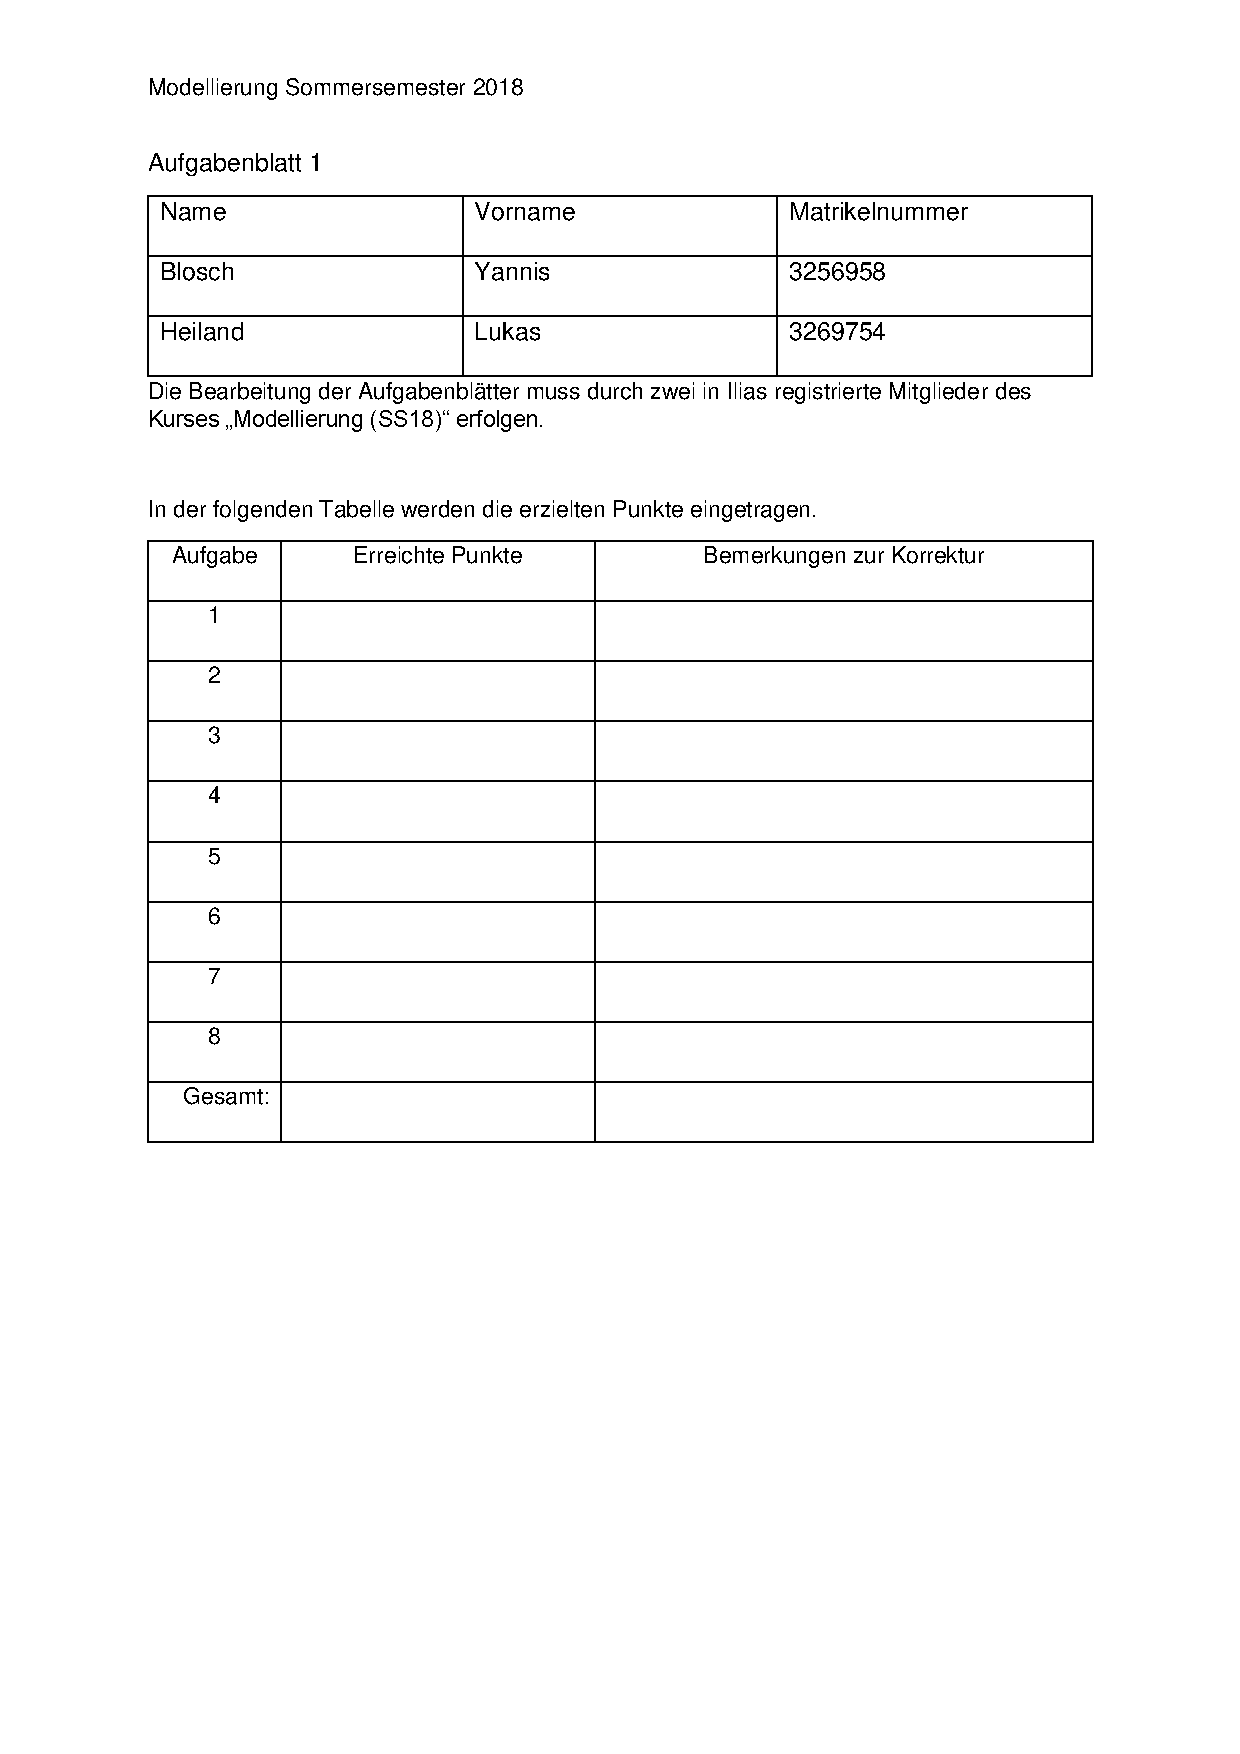
\includepdf[pages=-]{deckblatt.pdf}
	
	% Counter für das Blatt und die Aufgabennummer.
% Ersetze die Nummer des Übungsblattes und die Nummer der Aufgabe
% den Anforderungen entsprechend.
% Beachte:
% \setcounter{countername}{number}: Legt den Wert des Counters fest
% \stepcounter{countername}: Erhöht den Wert des Counters um 1.
\newcounter{sheetnr}
\setcounter{sheetnr}{1} % Nummer des Übungsblattes
\newcounter{exnum}
\setcounter{exnum}{1} % Nummer der Aufgabe

% Befehl für die Aufgabentitel
\newcommand{\exercise}[1]{\section*{Aufgabe \theexnum\stepcounter{exnum} #1}} % Befehl für Aufgabentitel

% Formatierung der Kopfzeile
% \ohead: Setzt rechten Teil der Kopfzeile mit
% Namen und Matrikelnummern aller Bearbeiter
\ohead{Yannis Blosch (3256958)\\
Lukas Heiland (3269754)}
% \chead{} kann mittleren Kopfzeilen Teil sezten
% \ihead: Setzt linken Teil der Kopfzeile mit
% Modulnamen, Semester und Übungsblattnummer
\ihead{Modellierung\\
Sommersemester 2018\\
Blatt \thesheetnr}
	
	\section*{Aufgabe 1.1}
		\paragraph{TODO}
		
	\section*{Aufgabe 1.2}
		%%% Aufgabenteil a (LHE)
		\subsection*{a.}
		.
			\begin{figure}[h]
				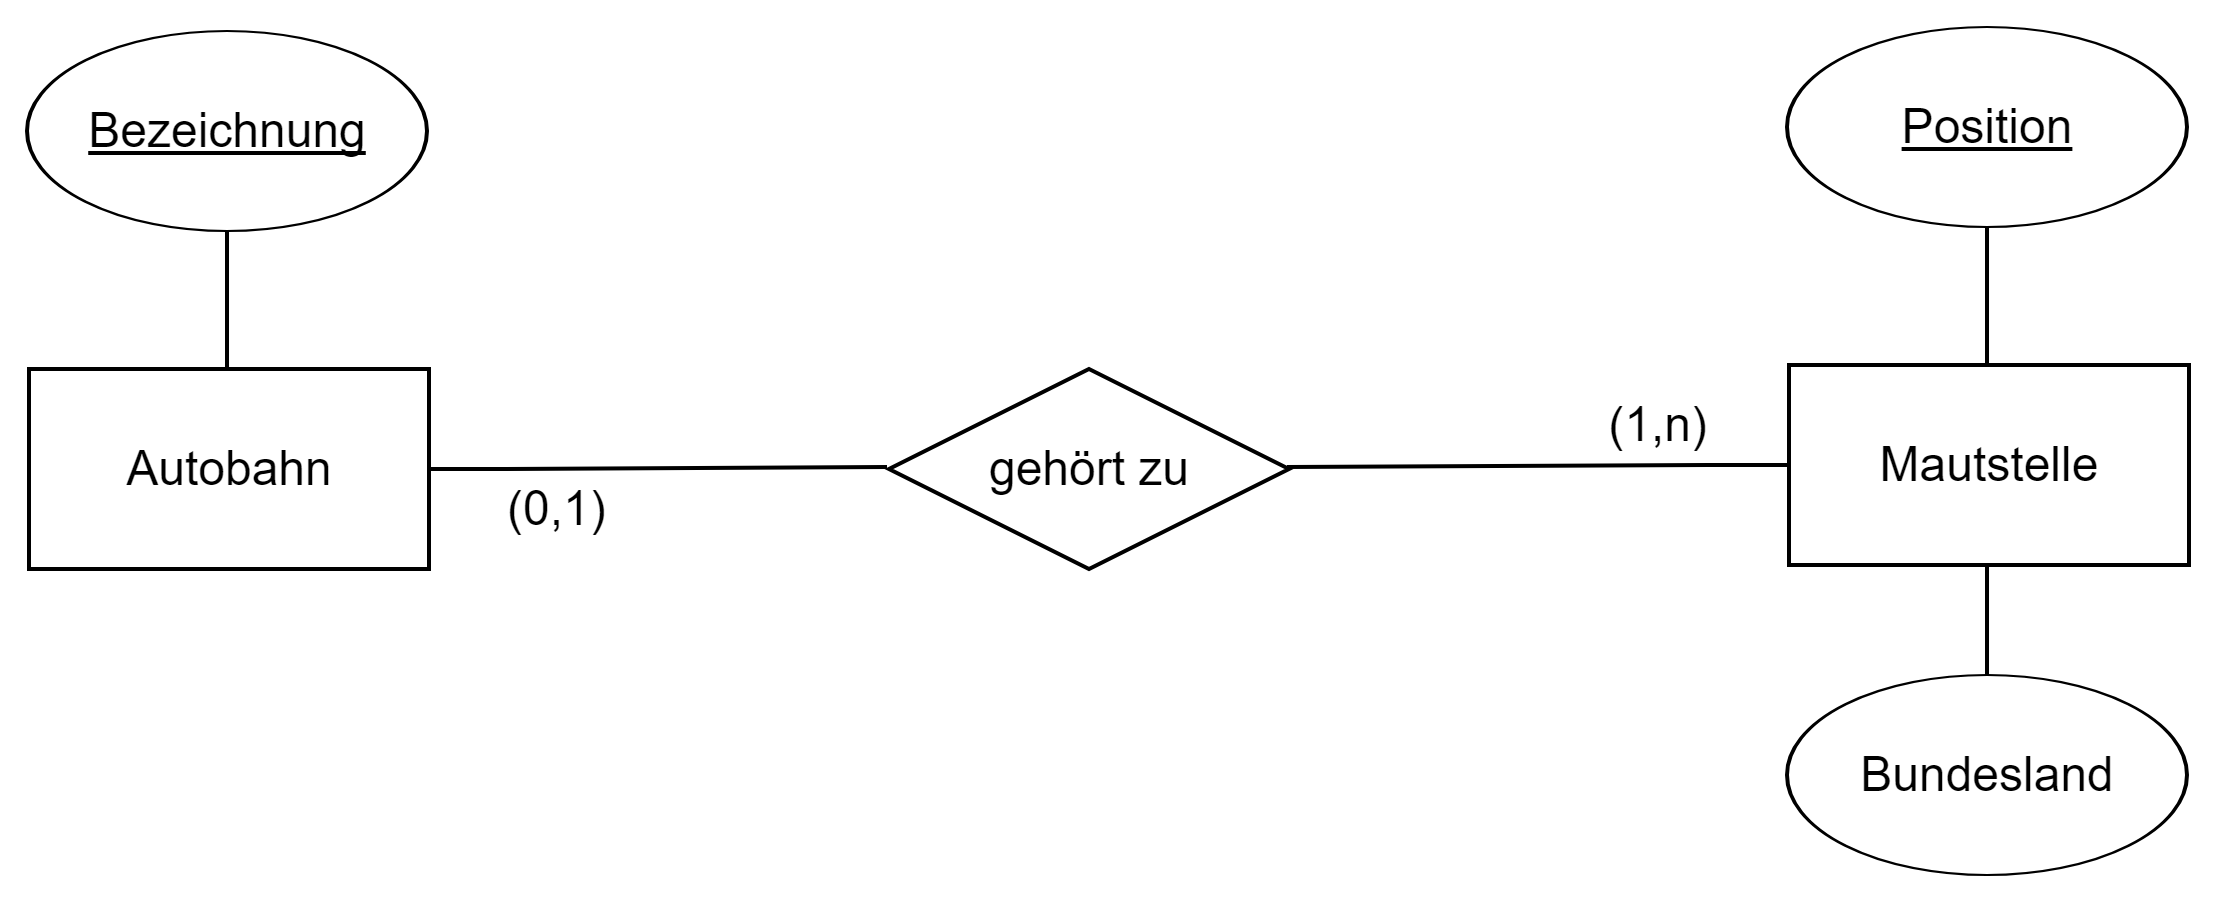
\includegraphics[width=0.7\textwidth]{aufgabe_1_2_a.png}
			\end{figure}
		
		%%% Aufgabenteil b (YBL)
		
		
		%%% Aufgabenteil c (LHE)
		\subsection*{c.}
		.
			\begin{figure}[h]
				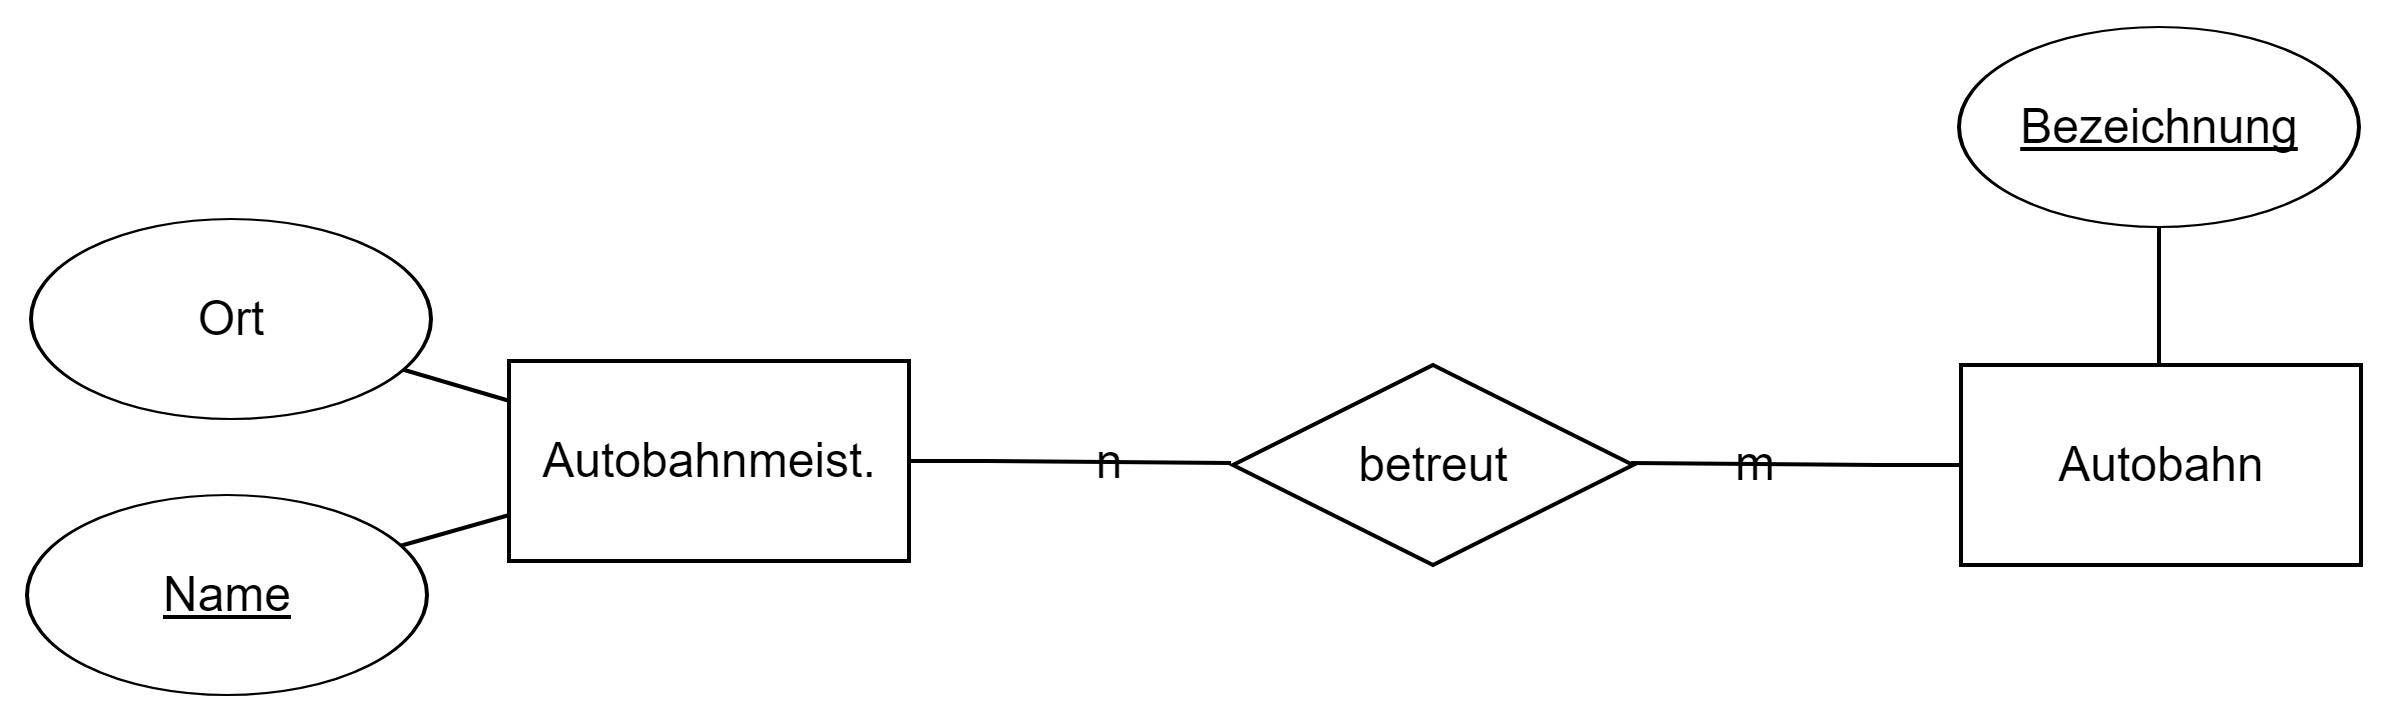
\includegraphics[width=0.7\textwidth]{aufgabe_1_2_c.png}
			\end{figure}
			
		
		%%% Aufgabenteil d (YBL)
		
		
		%%% Aufgabenteil e (LHE)
		\subsection*{e.}
		.
			\begin{figure}[h]
				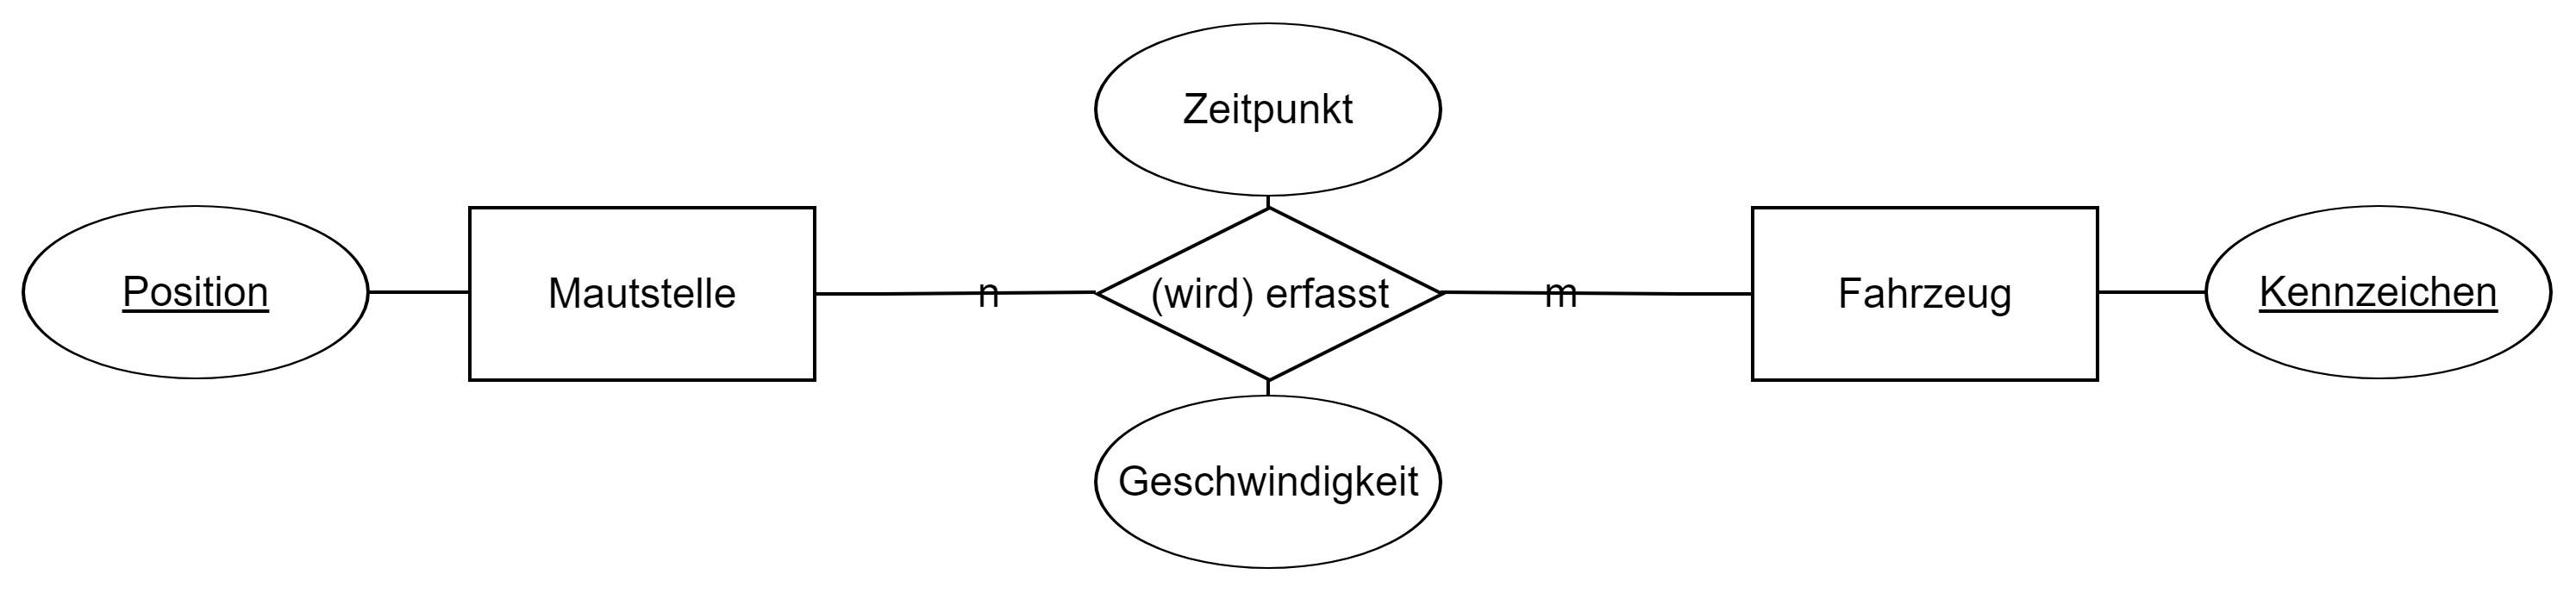
\includegraphics[width=0.7\textwidth]{aufgabe_1_2_e.png}
			\end{figure}
		
		%%% Aufgabenteil f (YBL)
		
		
		
		%%% layout reasons
		\pagebreak
		
		%%% Aufgabenteil g (LHE)
		\subsection*{g.}
		.
			\begin{figure}[h]
				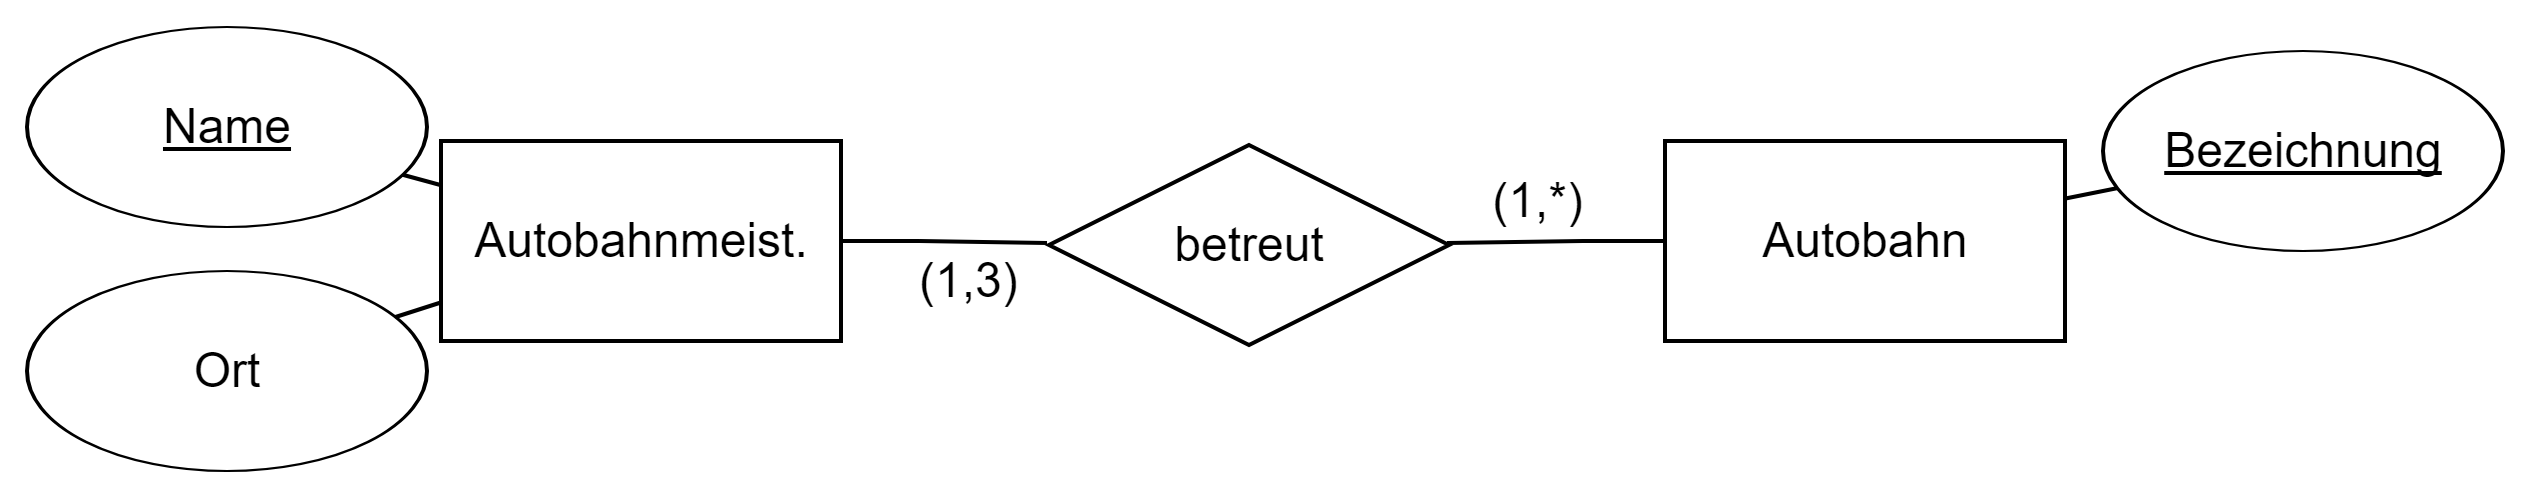
\includegraphics[width=0.7\textwidth]{aufgabe_1_2_g.png}
			\end{figure}
		
		%%% Aufgabenteil h (YBL)
		
		
\end{document}